\documentclass[a4paper,10pt]{article}

\usepackage[T1]{fontenc}
\usepackage[utf8]{inputenc}
\usepackage{graphicx}
\usepackage{xcolor}
\usepackage{fourier}
\usepackage{caption}
\usepackage{subcaption}
\usepackage{cprotect}

\usepackage{tgtermes}

\usepackage[
pdftitle={Statistical Machine Learning}, 
pdfauthor={Inez Wijnands \& Guido Zuidhof, Radboud University Nijmegen},
colorlinks=true,linkcolor=blue,urlcolor=blue,citecolor=blue,bookmarks=true,
bookmarksopenlevel=2]{hyperref}
\usepackage{amsmath,amssymb,amsthm,textcomp}
\usepackage{enumerate}
\usepackage{multicol}
\usepackage{tikz}

\usepackage{geometry}
\geometry{total={210mm,297mm},
left=25mm,right=25mm,%
bindingoffset=0mm, top=20mm,bottom=20mm}

\numberwithin{equation}{section} % Number equations within sections (i.e. 1.1 instead of 1)
\numberwithin{figure}{section} % Number figures within sections (i.e. 1.1 i/o 1)
\numberwithin{table}{section} % Number tables within sections (i.e. 1.1 i/of 1)

\linespread{1.35}

\newcommand{\linia}{\rule{\linewidth}{0.5pt}}

% custom theorems if needed
\newtheoremstyle{mytheor}
    {1ex}{1ex}{\normalfont}{0pt}{\scshape}{.}{1ex}
    {{\thmname{#1 }}{\thmnumber{#2}}{\thmnote{ (#3)}}}

\theoremstyle{mytheor}
\newtheorem{defi}{Definition}

% my own titles
\makeatletter
\renewcommand{\maketitle}{
\begin{center}
\vspace{2ex}
{\huge \textsc{\@title}}
\vspace{1ex}
\\
\linia\\
\@author  \@date
\vspace{4ex}
\end{center}
}
\makeatother
%%%

% custom footers and headers
\usepackage{fancyhdr,lastpage}
\pagestyle{fancy}
\lhead{}
\chead{}
\rhead{}
\lfoot{Assignment \textnumero{} 3}
\cfoot{}
\rfoot{Page \thepage\ /\ \pageref*{LastPage}}
\renewcommand{\headrulewidth}{0pt}
\renewcommand{\footrulewidth}{0pt}
%

% code listing settings
\usepackage{listings}
\lstset{
    language=Python,
    basicstyle=\ttfamily\small,
    aboveskip={0.9\baselineskip},
    belowskip={0.9\baselineskip},
    columns=fixed,
    extendedchars=true,
    breaklines=true,
    tabsize=4,
    prebreak=\raisebox{0ex}[0ex][0ex]{\ensuremath{\hookleftarrow}},
    frame=lines,
    showtabs=false,
    showspaces=false,
    showstringspaces=false,
    keywordstyle=\color[rgb]{0.1,0.126,0.941},
    commentstyle=\color[rgb]{0.133,0.545,0.133},
    stringstyle=\color[rgb]{0,0.5,0},
    numbers=left,
    numberstyle=\scriptsize\ttfamily,
    stepnumber=1,
    numbersep=10pt,
    captionpos=t,
    escapeinside={\%*}{*)}
}

%%%----------%%%----------%%%----------%%%----------%%%

\begin{document}

\title{Statistical Machine Learning \\ Assignment 3}

\author{Inez Wijnands (s4149696) \& Guido Zuidhof (s4160703)\\ Radboud University Nijmegen\\}

\date{03/12/2015}

\maketitle

\noindent \textit{The entire code listing is included in the zip-file. The listings shown here are merely code snippets}.\vspace{-0.5cm}
\section{Bayesian linear regression}
\begin{enumerate}
	\item \begin{align}
		\{x_1,t_1\} &= (0.4, 0.05)\\
		\{x_2,t_2\} &= (0.6, -0.35)\\
		\alpha &= 2\\
		\beta &= 10\\
		\end{align}
		\noindent We need to compute the predictive distribution $p(t | x,\boldsymbol{t},\boldsymbol{x}, \alpha, \beta)$ after the two data points (where $x$ is the input and $t$ is the target) are observed.\\\\
		\textbf{Step 1:} Identify the vector of basis functions $\phi(\boldsymbol{x})$, and write out $\boldsymbol{\Phi}^T\boldsymbol{t}$ and $\boldsymbol{\Phi}^T\boldsymbol{\Phi}$ in terms of the data $\{x_n,t_n\}$.
		\begin{align}
		\boldsymbol{\Phi}^T\boldsymbol{t} &= \sum_n \boldsymbol{\phi}(x_n)t_n = N\begin{pmatrix} \bar{\mu}_t \\ \bar{\mu}_{xt}\end{pmatrix}\\
		\boldsymbol{\Phi}^T\boldsymbol{\Phi} &= \sum_n \boldsymbol{\phi}(x_n)\boldsymbol{\phi}(x_n)^T = N\begin{pmatrix} 1 & \bar{\mu}_x \\ \bar{\mu}_x & \bar{\mu}_{xx} \end{pmatrix}
		\end{align}
		Where: 
		\begin{align*}
		\bar{\mu}_t = \frac{1}{N} \sum_n t_n  & &  \bar{\mu}_{xt} = \frac{1}{N} \sum_n x_nt_n \\
		\bar{\mu}_x = \frac{1}{N} \sum_n x_n & & \bar{\mu}_{xx} = \frac{1}{N} \sum_n x_n^2
		\end{align*}
		Combined:
		\begin{align}
		\boldsymbol{\Phi}^T\boldsymbol{t} &= \sum_n \boldsymbol{\phi}(x_n)t_n = N\begin{pmatrix} \bar{\mu}_t \\ \bar{\mu}_{xt}\end{pmatrix}\\
		& = N\begin{pmatrix} \frac{1}{N} \sum_n t_n \\ \frac{1}{N} \sum_n x_nt_n\end{pmatrix} \\
		& = 2\begin{pmatrix} \frac{1}{2} (0.05 + -0.35) \\ \frac{1}{2} (0.4\cdot 0.05 + 0.6 \cdot -0.35)\end{pmatrix} \\
		& = \begin{pmatrix} -0.3 \\  -0.19 \end{pmatrix}
		\end{align}
		\begin{align}
		\boldsymbol{\Phi}^T\boldsymbol{\Phi} &= \sum_n \phi(x_n)t_n = N\begin{pmatrix} 1 & \bar{\mu}_x \\ \bar{\mu}_x & \bar{\mu}_{xx} \end{pmatrix}\\
		& = N\begin{pmatrix} 1 & \frac{1}{N} \sum_n x_n \\ \frac{1}{N} \sum_n x_n & \frac{1}{N} \sum_n x_n^2 \end{pmatrix}\\
		& = 2\begin{pmatrix} 1 & \frac{1}{2} (0.4 + 0.6) \\ \frac{1}{2} (0.4 + 0.6) & \frac{1}{2} (0.4^2 + 0.6^2) \end{pmatrix}\\
		& = \begin{pmatrix} 2 & 1 \\ 1 & 0.52 \end{pmatrix}
		\end{align}\\
		\textbf{Step 2:} Compute the posterior $p(\boldsymbol{w} | \boldsymbol{t}, \boldsymbol{x}, \alpha, \beta)$. 
		\begin{align}
		p(\boldsymbol{w} | \alpha) &= \mathcal{N}(\boldsymbol{w} | 0, \alpha^{-1}\boldsymbol{I})\\
		p(\boldsymbol{t} | \boldsymbol{w}, \boldsymbol{x}) &= \mathcal{N}(\boldsymbol{t} | \boldsymbol{\Phi}\boldsymbol{w}, \beta^{-1}\boldsymbol{I})\\
		&\rightarrow\\
		p(\boldsymbol{w} | \boldsymbol{t}, \boldsymbol{x}) &= \mathcal{N}(\boldsymbol{w} | \boldsymbol{m}_N, \boldsymbol{S}_N)\\	
		\boldsymbol{S}_N^{-1} &= \alpha \boldsymbol{I} + \beta \boldsymbol{\Phi}^T\boldsymbol{\Phi} = \begin{pmatrix} \alpha & 0 \\ 0 & \alpha \end{pmatrix} + N\beta \begin{pmatrix} 1 & \bar{\mu}_x \\ \bar{\mu}_x & \bar{\mu}_{xx} \end{pmatrix}\\
		&= \begin{pmatrix} 2 & 0 \\ 0 & 2 \end{pmatrix} + 10 \begin{pmatrix} 2 & 1 \\ 1 & 0.52 \end{pmatrix}\\
		&=  \begin{pmatrix} 2 & 0 \\ 0 & 2 \end{pmatrix} + \begin{pmatrix} 20 & 10 \\ 10 & 5.2 \end{pmatrix} \\
		&=  \begin{pmatrix} 22 & 10 \\ 10 & 7.2 \end{pmatrix}\\
		\boldsymbol{m}_N &= \beta \boldsymbol{S}_N \boldsymbol{\Phi}^T\boldsymbol{t} = N\beta \boldsymbol{S}_N \begin{pmatrix} \bar{\mu}_t \\ \bar{\mu}_{xt} \end{pmatrix}\\
		&= 10 \begin{pmatrix} 22 & 10 \\ 10 & 7.2 \end{pmatrix}^{-1} \begin{pmatrix} -0.3 \\  -0.19 \end{pmatrix} \\
		&= \begin{pmatrix} -0.0445 \\  -0.2021 \end{pmatrix}
		\end{align}\\
		\textbf{Step 3:} Compute the predictive distribution $p(t | x,\boldsymbol{t},\boldsymbol{x}, \alpha, \beta) = \mathcal{N}(t | m(x), s^2(x))$ in terms of known or computable quantities, we do this the same way as we obtained the posterior distribution in step 2.
		\begin{align}
		p(\boldsymbol{w} | \boldsymbol{t},\boldsymbol{x}) &= \mathcal{N}(\boldsymbol{w}|\boldsymbol{m}_N, \boldsymbol{S}_N)\\
		p(t | \boldsymbol{w}, \boldsymbol{t}, \boldsymbol{x}) &= \mathcal{N}(t | \boldsymbol{\phi}(x)^T\boldsymbol{w}, \beta^{-1}\\
		&\rightarrow\\
		p(t | x, \boldsymbol{t}, \boldsymbol{x}) &= \mathcal{N}(t | \boldsymbol{m}_N^T \boldsymbol{\phi}(x), \sigma_N^2(x))
		\end{align}
		With $\boldsymbol{m}_N$ and $\boldsymbol{S}_N$ defined as before, and
		\begin{align}
		\sigma_N^2(x) &= \frac{1}{\beta} + \boldsymbol{\phi}(x)^T\boldsymbol{S}_N\boldsymbol{\phi}(x)
		\end{align}
		\begin{align}
		p(t | x, \boldsymbol{t},\boldsymbol{x}, \alpha, \beta) &= \mathcal{N}(t | m(x), s^2(x))\\
		m(x) &= \boldsymbol{m}_N^T \boldsymbol{\phi}(x)\\
		&= \begin{pmatrix} -0.0445 \\ -0.2021 \end{pmatrix}^T \begin{pmatrix} 1 \\ x \end{pmatrix}\\
		s(x) &= \sigma_N^2\\
		&= \frac{1}{10} + \begin{pmatrix} 1 \\ x \end{pmatrix}^T \begin{pmatrix} 22 & 10 \\ 10 & 7.2 \end{pmatrix}^{-1} \begin{pmatrix} 1 \\ x \end{pmatrix}
		\end{align}
	\item See Figure 1.1 where the mean of the predictive Gaussian distribution and one standard deviation on both sides are plotted as a function over $x$ over the interval $[0,1]$, with the two observed data points. When we compare this plot with Figure 3.8b (Bishop, p.157), is our linear mean. This can be explained by the nature of our basis function $\phi_j$, which is two-dimensional in our case and Bishop uses a 9-dimensional function.
		\begin{figure}[h]
   			\centering
   			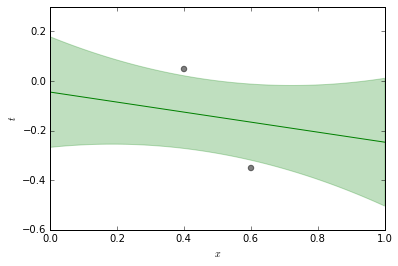
\includegraphics[width=0.95\textwidth]{exercise1plottanopink.png}\vspace{-0.4cm}
   			\caption{\vspace{-0.1cm} The mean of the predictive Gaussian distribution is represented by the green line, plotted against $x$. \vspace{-0.1cm}The two grey dots are the data points $\{x_1,t_1\}$ and $\{x_2,t_2\}$. The light green area indicates the standard deviation and is bound by the mean plus the standard deviationd and the mean minus the standard deviation.}\vspace{-0.2cm}
  		\end{figure}
	\item We sampled five functions $y(x, \boldsymbol{w})$ from the posterior distribution over $\boldsymbol{w}$ (see Exercise 1.1 step 2) for this data set and plotted them with the predictive distribution (see Figure 1.2). 
		\begin{figure}[h!]
   			\centering
   			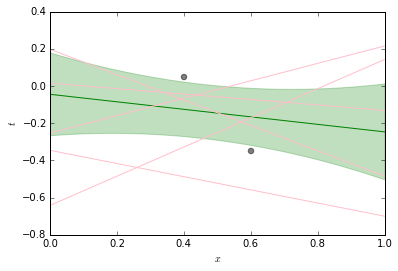
\includegraphics[width=0.95\textwidth]{exercise1plotta.png}\vspace{-0.4cm}
   			\caption{\vspace{-0.0cm} The pink lines represent $y(x,\boldsymbol{w})$ where the weights $\boldsymbol{w}$ are sampled from the posterior distribution with mean $m_N$ and variance $S_N$.}
  		\end{figure}
\end{enumerate}

\vfill 

\section{Logistic regression}
\subsection{The IRLS algorithm}
\begin{enumerate}
	\item 
	\item 
	\item 
\end{enumerate}

\subsection{Two-class classification using logistic regression}
\begin{enumerate}
	\item 
\end{enumerate}
\end{document}
